
\section{Maxwell's Equations}
Dr. Butler recommends reading the Maxwell review on Blackboard (\href{https://ualearn.blackboard.com/bbcswebdav/pid-3974540-dt-content-rid-36341461_1/courses/11111.201910/Reading\%20Assingnments/Review\%20of\%20Maxwell\%27s\%20Equations\%281\%29.pdf}{link}).


\subsection{WHB Pedagogical Transformations}
Dr. Butler does not think the way Griffiths presents Maxwell's equations is the best. Dr. Butler likes to write them in terms of the electric field $\mathbf{E}$ and magnetic field $\mathbf{H}$, and relate these to the electric flux density $\mathbf{D}$ and $\mathbf{B}$ with the polarization $\mathbf{P}$ and magnetization $\mathbf{M}$. They turn into the following

    \begin{align*}
        \diver \mathbf{E} &= \frac{\rho_e}{\epsilon_0} & -\curl \mathbf{E} = \mathbf{J}_m + \diff{\mathbf{B}}{t} \\
        \diver \mathbf{H} &= \frac{\rho_m}{\mu_0} & \curl \mathbf{H} = \mathbf{J}_e + \diff{\mathbf{D}}{t}
    \end{align*}
    
with $\rho_m$ being the "magnetic charge" and $\mathbf{J}_m$ being the "magnetic current." These are related to the flux densities by (Butler's magnetization to Griffiths is: $\mathbf{M}'=\mu_0 \mathbf{M}$)
    \begin{align*}
        \mathbf{D} = \epsilon_0 \mathbf{E} + \mathbf{P} \hspace{20pt}    \mathbf{B} = \mu_0 \mathbf{H} + \mathbf{M}' \\
    \end{align*}
    
\emph{Should know how to transform to Griffiths form.}

\textbf{Charge densities with media:}
    \begin{align*}
        \diver \mathbf{D} &=  \epsilon_0 \diver \mathbf{E} + \diver \mathbf{P} & \diver \mathbf{B} &= \mu_0 \diver \mathbf{H} + \diver \mathbf{M}' \\
        \rho_{ef} &= \rho_e - \rho_{eb} & \rho_{mf} &= \rho_m - \rho_{mb} 
    \end{align*}
    
\subsection{Experimental Basis for Maxwell Equations}
Dr. Butler (and many other professors) have emphasized the experimental basis of these equations. He expects us to know them.

\subsubsection{Coulomb's Potentials}
% ADD DERIVATION AND MAYBE DIAGRAM
Coulomb's experiments in the 18th century imply both divergence equations. The experiment measured the proportionality between the fields and the amount of charge for electric charges and magnetic poles. This inverse square relation with a Green's function and the divergence theorem gives the divergence equations.
    \begin{align*}
        \diver \mathbf{E} = \frac{\rho_e}{\epsilon_0} \hspace{20pt} \diver \mathbf{H} = \frac{\rho_m}{\mu_0} \\
    \end{align*}

\begin{figure}[!hbtp]
    \centering
    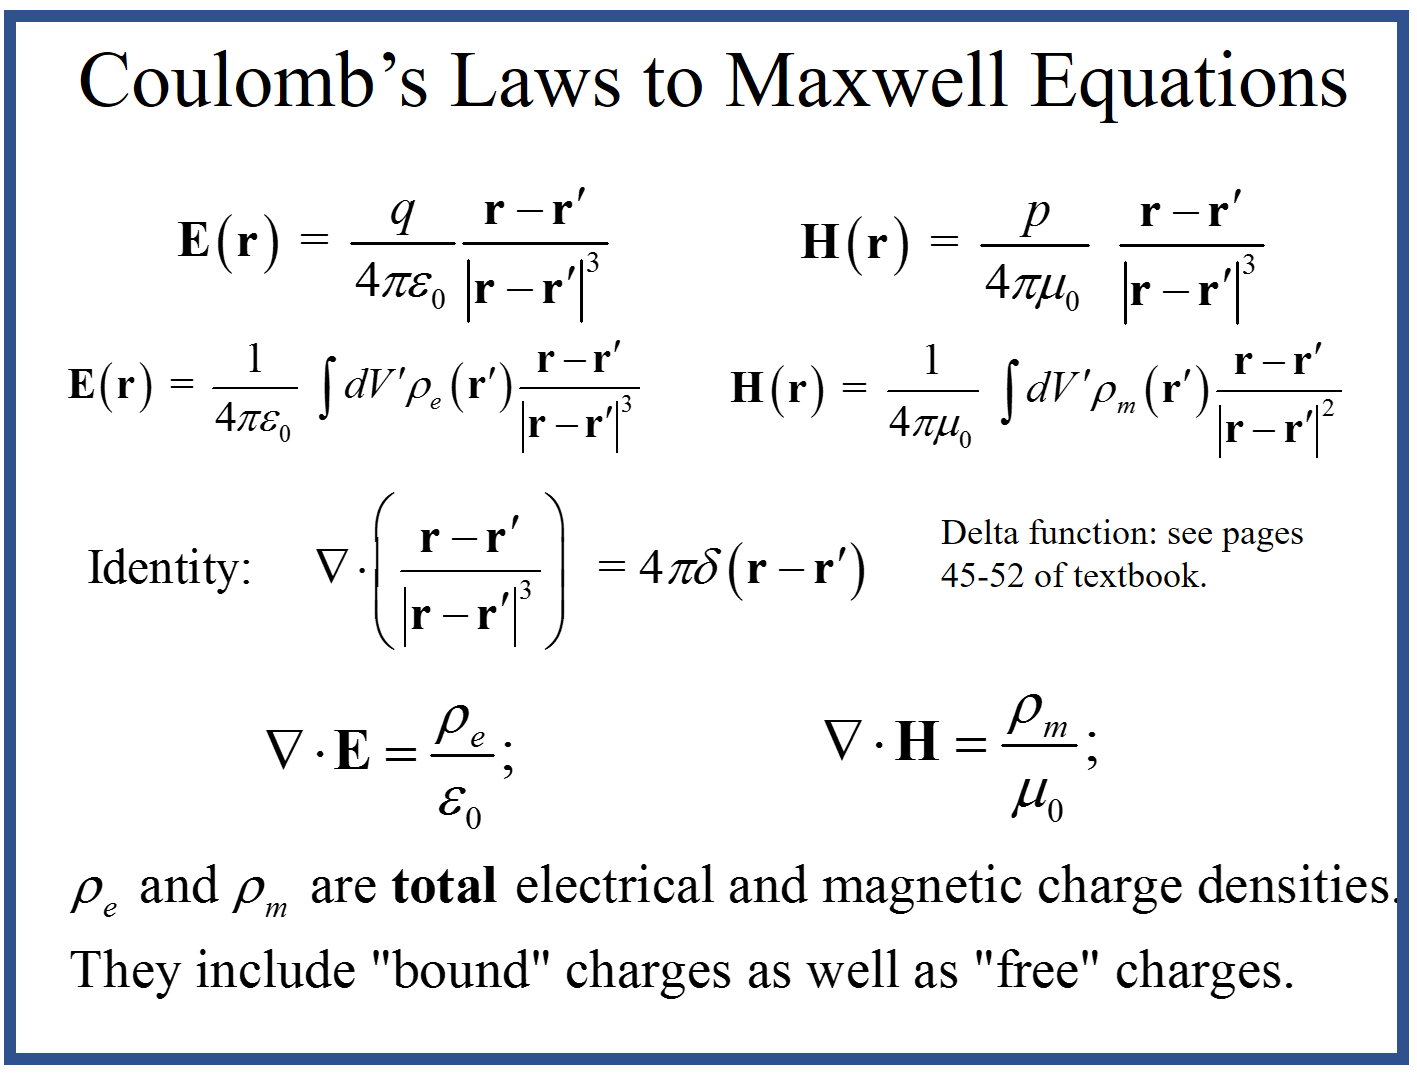
\includegraphics[scale=.2]{Images/coloumb.png}
    \caption{Derivation of Divergence Laws from Coulomb experiments.}
    \label{fig:coulomb}
\end{figure}

\subsubsection{Ampere's Law}
% FILL
Ampere observed 
\textcolor{orange}{UNDER CONSTRUCTION.}


\subsubsection{Maxwell Correction}
% FILL
\textcolor{orange}{UNDER CONSTRUCTION.}


\subsubsection{Faraday's Experiments}
% FILL
\textcolor{orange}{UNDER CONSTRUCTION.}